\documentclass[12pt]{article}
\usepackage{graphicx} % Required for inserting images
\usepackage{hyperref}

\title{Mini Gaming Hub - Project Report}
\author{Araveti Satya Sai Shabarish \& Pedda Venkata Karthik}

\begin{document}

\maketitle

\section{External Libraries/Tools}
\label{sec:ELT}
\subsection{External Libraries}
\begin{enumerate}
    \item Numpy - used in games to check win condition
    \item Matplotlib - to draw the pie chart to show the popularity of games and bar graph to show the top 5 players
    \item pygame-ce - for GUI
\end{enumerate}
\subsection{External Tools}
\begin{enumerate}
    \item grep - to check if the conditions for the username and password are met
    \item sha256sum - to hash the password entered by the user
    \item awk - to format the lines in leaderboard and break the lines into fields, using delimiter
\end{enumerate}

\section{Design \& Architecture}

\subsection{Connection}
\textbf{game.py} is the heart of the project, everything is connected to game.py
\begin{enumerate}
    \item game.py contains the class which is inheritable, containing the common methods \& variables for all the games
    \item game.py imports the play\_game() function from other files in the games folder, to prevent program from crashing we made everything into functions and called the main function at the end (so that it runs only when the bash script calls the game.py but not when other files imported)
    \item game.py also should show the charts and leaderboard, here subprocess is used to run those in different processes otherwise program would crash due to ghost clicks, due to pygame waiting for the previous process to stop,etc
    \item used many types of booleans to ensure that the unexpected clicks shall not affect the main-menu(ex:- when game is selected, LEADERBOARDS, ANALYTICS options shall not work)
\end{enumerate}

\subsection{Data handling}
\begin{enumerate}
    \item In main.sh we didn't allow username to be of length > 12 so that while rendering the username anywhere in the GUI it doesn't become ugly
    \item writing the status to the history.csv(first column), so that we know if the game is Draw
    \item We used the status of the function wherever necessary so that the consequences will be based on those status(ex:- play\_game returns 1/2 if the game is played till end, 3 if the game is exits while loading)
    \item used the associative arrays in the leaderboard.sh so that we don't use many variables unneccessarily, this array infact acts like 3d array
\end{enumerate}


\section{Features Implemented}
\begin{itemize}
    \item Main-Menu offers 3 games which can be selected
    \item Exit option - Allows user to exit anytime from the main-menu and the loading page
    \item Quit option - Allows user to quit from the game leading to opposite player to win
    \item A Drop down Sortby - Allows user to choose the metric by which the leaderboard should be sorted by
    \item ANALYTICS option - Allows user to look at the graphs/charts at anytime
    \item LEADERBOARDS option - Allows user to look at the leaderboard at anytime(including the draw option)
    \item pop-up appears after selecting the game - Allows to select whose turn is the first, it blinks if you try to select other options, meaning you can't exit at that point
    \item while playing the game users can look at the colours which they were assigned to
    \item othello game lets you know the valid moves for easy gameplay
    \item connect4, tictactoe games lets you know how the player won, by drawing a line
    \item every game lets you know which player won the match (or draw match)
    \item after every gameplay, returns to the main-menu, a pop-up appears asking if the users wants to quit
\end{itemize}
\clearpage
\section{Directory Structure}
\begin{verbatim}
    CS108-PROJECT/
                |--games/
                    |--othello.py
                    |--tictactoe.py
                    |--connect4.py
                |--main.sh
                |--leaderboard.sh
                |--game.py
                |--analysis.py
                |--Makefile
                |--report.tex
                |--report.pdf
                |--users.tsv
                |--history.csv

\end{verbatim}
\begin{itemize}
    \item games - folder in which all the source code and images related to playing the game are kept
    \item othello.py - source code to play the OTHELLO game
    \item tictactoe.py - source code to play the TIC-TAC-TOE game
    \item connect4.py - source code to play the CONNECT4 game
    \item main.sh - source code to regester/authenticate the user
    \item leaderboard.sh - source code to display the leaderboards of the games played till the moment
    \item game.py - connects all the games and main-menu and contains the gui for the main-menu
    \item analysis.py - helper file to display the charts of matplotlib(ran using subprocess)
    \item Makefile - used to compile the latex file
    \item report.tex - source code to the report of the project
    \item report.pdf - contains the report of the project
    \item users.tsv - contains the usernames and hashed passwords of the users of the Gaming Hub
    \item history.csv - contains the data of the all games played till the moment in the Hub
\end{itemize}

\section{Installation \& Setup}
To run the game you shall first install the external Libraries/Tools required, checkout Section \ref{sec:ELT} \\
Assuming you are using python3.10 version and linux environment \\
For clean setup using virtual environment, first activate it and then run
\begin{enumerate}
    \item  \texttt{python3 -m pip install --upgrade pip}
    \item  \texttt{python3 -m pip install pygame-ce matplotlib numpy} 
\end{enumerate}
Generally external tools are already installed in your system but still if you face any issues then run
\begin{enumerate}
    \item  \texttt{sudo apt install coreutils grep gawk}
\end{enumerate}
\section{Usage}
In the terminal run \texttt{bash main.sh}, you will get this output \\
\begin{figure}[h!]
    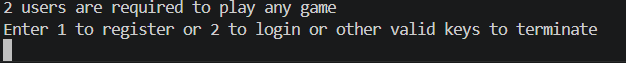
\includegraphics[width=\textwidth]{BS.png}
\end{figure}
you have to press only 1 or 2 other numbers/alphabets terminate the script
If you want to regester give a username and password(there are few conditions to met, you can see them as you try to register) and you can later login, or if you want to login you can directly login with correct username and password combination \\
But you can not play the games until \textbf{2} users logged in \\
After 2 players are logged in you will see the following image with a new window opened(closing leads to termination of the entire project)\\
\begin{figure}[ht]
    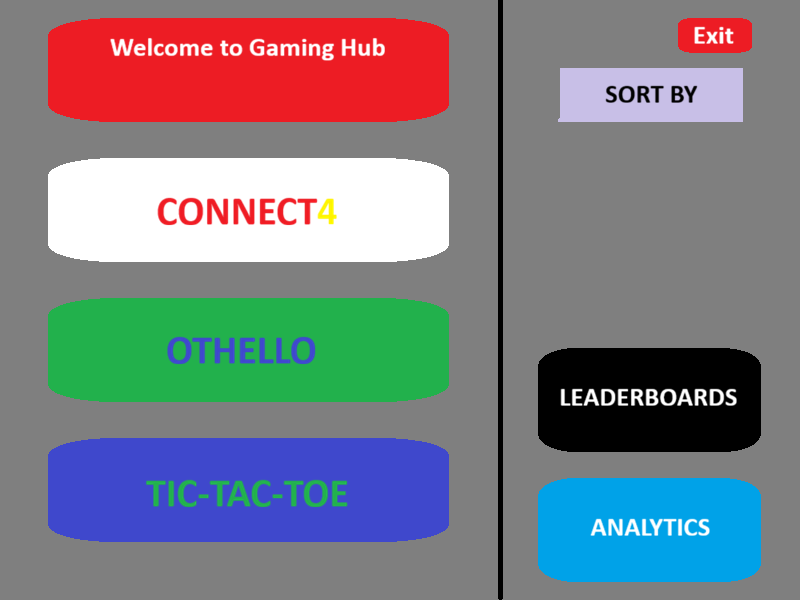
\includegraphics[width=\textwidth]{MWS.png}
\end{figure}
But with the usernames displayed above(in the red region)\\
Select any game to play or select ANALYTICS to view the charts or select LEADERBOARDS to view the leaderboard in the terminal, you can also exit by clicking the exit option(project terminates)\\
You can choose any metric in by selecting the 'Sort By' dropdown to sort the leaderboard\\ 
Click on any game you will be presened with a pop-up asking if the user with the username mentioned in the pop-up wanted to make first move \\
At this point you can't exit, you shall play\\
after selecting any option you can see a loading page for the game you selected there you can exit(Quit option)\\
When game starts you can play or quit(if you quit you lose the match)\\
After gameplay you are presented with a figure containing charts, graphs and also leaderboard in the terminal\\
You are asked if you want to continue playing or quit(a pop-up appears) like this\\
\begin{figure}[ht]
    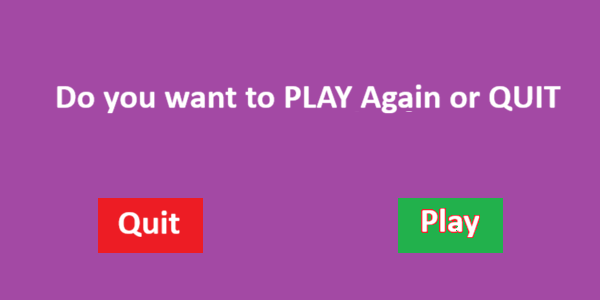
\includegraphics[width=\textwidth]{EP.png}
\end{figure}
If you quit all the project terminates, else you will be returned to main-menu\\ \\
HAVE FUN PLAYING THE GAMES

\section{Retrospective}

\subsection{Challenges}
\begin{itemize}
    \item in leaderboard.sh sorting the win/lose ratio, as it was including text with numbers using awk and few other files to store temporary info helped
    \item in leaderboard.sh maintaining vast info of games, users, win/lose/draw counts - using 1d associative arrays as 3d arrays by giving games, metrics ID helped
    \item in main.sh finding if the user met the conditions of username, password - using 1 or more grep in the if conditions helped
    \item in game.py and allover the games source codes managing the screen object - sending as an argument helped a lot
    \item getting a conclusion to make a common class based on the games code my partner written - not one thing spend 3 days to understand it and write a common class
    \item while running the code leaderboard, charts in different scripts may crash the program - used subprocess to run it in an entirely different process
    \item changing the 'Sort By' option as dropdown menu - updating the images and also updating the display helped
    \item drawing the line after winning in TIC-TAC-TOE and CONNECT4 - understanding the drawline function properly and drew accordingly
    \item clicking somewhere on the screen(except board) is leading to the placing move - limiting the co-ordinates (x-axis) to only board
    \item Valid moves in the OTHELLO - Checking 8 directions, if the move leads to sandwich, created a function check\_direction, to check whether if it is sandwiched, and function valid-move, to check all 8 directions using check-direction function and return if any 1 of it results to true
    \item Flipping the opponent pieces - making a list 'cells' which stores the cell co-ordinated which are to be flipped
\end{itemize}
\subsection{What if we got more time}
\begin{itemize}
    \item Restart option- while playing the game if the users wanted to play from the beginning without completing the game
    \item Making main-menu, games display much more engaging and after game completion displaying winner with big font size and with different colours
    \item Adding help option - to show the instructions \& rules for the gameplay
\end{itemize}
\end{document}
